\documentclass[11pt]{article}

\usepackage{amsmath}
\usepackage{hyperref}
\usepackage{graphicx}

\usepackage{titling}
\newcommand{\subtitle}[1]{%
  \posttitle{%
    \par\end{center}
    \begin{center}\large#1\end{center}
    \vskip0.5em}%
}




% %%%%%%%%%%%%%%%%%%%%%%%%%%%%%%%%%%%%%%%%%%%%%%%%%%%%%%%%%%
% SET THE TITLE
% %%%%%%%%%%%%%%%%%%%%%%%%%%%%%%%%%%%%%%%%%%%%%%%%%%%%%%%%%%

\title{Tweet Sentiment Extraction}
\subtitle{Udacity ML Engineer Capstone Project}
\author{Brull Borràs, Pere Miquel}
   
\date{\today}

\begin{document}
\maketitle

% --------------------
\section{Domain Background}
% --------------------

Data is all around us, and with the introduction of Social Networks, the most straight forward to share this data is via text. This means that we need to find ways to interpret unstructured and free information such as \textbf{language}. When being introduced into \textbf{Natural Language Processing}, Sentiment Analysis is the go-to example one would try to tackle in the form of \textit{tweets}. The statement behind it revolves around inferring if a rather short message could be classified as positive, negative or neutral, based on the subjective information of the language: is the author using "\textit{good} or "\textit{bad}" words? Can we try to predict the emotional state of the author based on such small piece of information?

What we are going to do, however, is look at this same problem from a different perspective. Given the sentiment of the author, can we actually know which words make a message being positive or negative?

% --------------------
\section{Problem Statement}
% --------------------

Our main objective is exploring different NLP techniques that could aid us into finding which parts of the message transmit the \textit{sentiment} information and classify those into positive, negative or neutral. This study is based on the \href{https://www.kaggle.com/c/tweet-sentiment-extraction}{Kaggle's Tweet Sentiment Extraction} competition.

We are going to use the \href{https://www.kaggle.com/c/tweet-sentiment-extraction/data}{train data} from the Kaggle platform. As the submission to the competition is out of the scope, we are going to use this same dataset as training and validation with a 80 / 20 split.

The train data is composed by 27.486 rows with the following information:
\begin{itemize}
    \item textID - Unique identifier of the row
    \item text - Complete tweet
    \item selected text - The text that supports the tweet's sentiment. It is a subset of the \textit{text} feature containing one extract from a sentence. I.e., it does not contain independent words from different parts of the tweet.
    \item sentiment - The generated sentiment of the text, which can be \textit{positive}, \textit{negative} or \textit{neutral}.
\end{itemize}

An \textbf{example} of some positive data is the following:

\begin{verbatim}
  Oh! Good idea about putting them on ice cream.
\end{verbatim}

Which has the following selected text:

\begin{verbatim}
  Good
\end{verbatim}

% --------------------
\section{Evaluation Metrics}
% --------------------

A key point that we need to define is how are we going to score our predicted outputs. In order to do that we will use the \href{https://en.wikipedia.org/wiki/Jaccard_index}{Jaccard index}:

\[
J(A,B) = {{|A \cap B|}\over{|A \cup B|}} = {{|A \cap B|}\over{|A| + |B| - |A \cap B|}}
\]

In our case, the sets $A$ and $B$ are the two sentences which we are comparing after \textit{lemmatization}, so that words such as \textit{friend} and \textit{friendly} are treated as equal. Therefore, following the discussion on the example above, if we would have received the output

\begin{verbatim}
  Good idea
\end{verbatim}

instead of the real selected text

\begin{verbatim}
  Good
\end{verbatim}

The result of the Jaccard index would be:

\[
J(A,B) = {{\{\text{Good}\}}\over{\{\text{Good}, \text{idea}\}}} = 0.5
\]

This way we are penalizing scenarios where we are not finding out enough information or where we are considering too much words that could have been avoided.

% --------------------
\section{Exploratory Data Analysis}
% --------------------

In this section we are going to review the train data and try to answer the following questions:

\begin{itemize}
    \item Is the data well balanced?
    \item What are the most common words for each sentiment?
    \item Are there any differences in the length of the selected texts for each sentiment?
\end{itemize}

% --------------------
\subsection{Data Balance}
% --------------------

The first question is easy to solve. After reading the data we just need to show the grouped counts:


\begin{figure}[h]
\centering
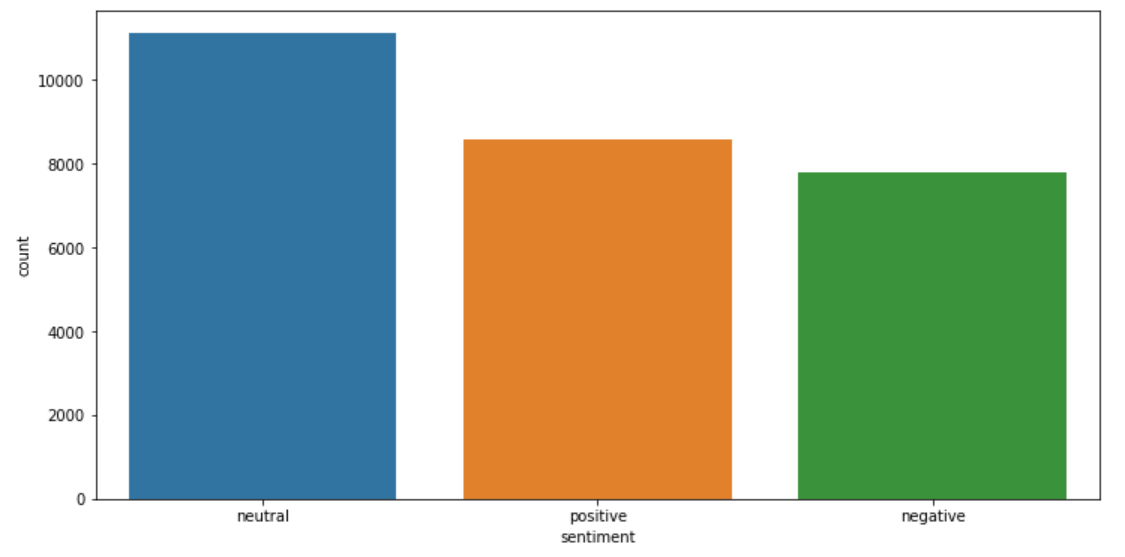
\includegraphics[width=12cm]{sentiment-distribution.png}
\caption{Sentiment distribution in the dataset}
\end{figure}


Based on the graphic, everything seems balanced enough. Let's also add the real values:

\begin{table}[h]
\centering
\begin{tabular}{l|l|l}
\hline
\hline
Neutral & Positive & Negative \\ \hline
11.117 & 8.582 & 7.786 \\ 
\hline
\hline
\end{tabular}
\caption{Sentiment count in the complete dataset}
\end{table}

% --------------------
\subsection{Most Common Words}
% --------------------

Checking the most common words is a great exercise to gain better understanding about the data we have at hand. For that, will first apply the preprocessing step to reduce variance and remove noise - meaningless words - and then extract the words that appear the most in the \textit{selected text} target.

However, before jumping right into the target, let's visualize some information regarding the words that are being used in the text input:



\begin{figure}[h]
\centering
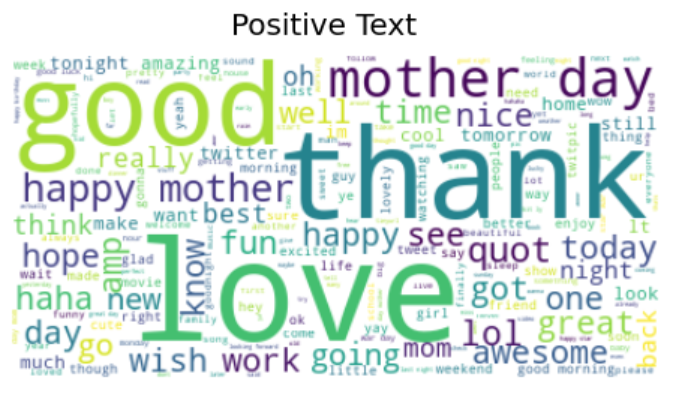
\includegraphics[width=8cm]{positive_text_wc.png}
\caption{Positive Text WordCloud}
\end{figure}



\begin{figure}[h]
\centering
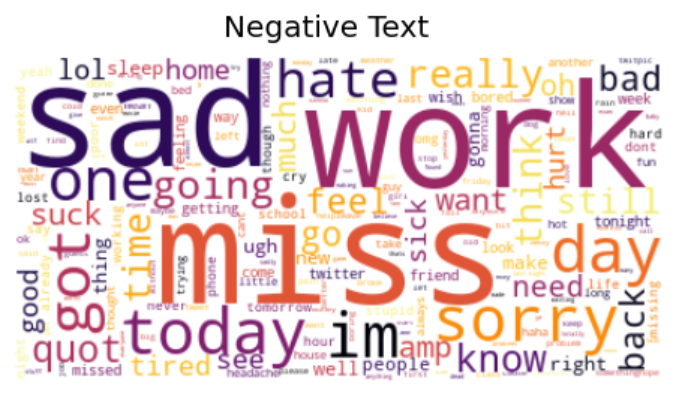
\includegraphics[width=8cm]{negative_text_wc.png}
\caption{Negative Text WordCloud}
\end{figure}



\begin{figure}[h]
\centering
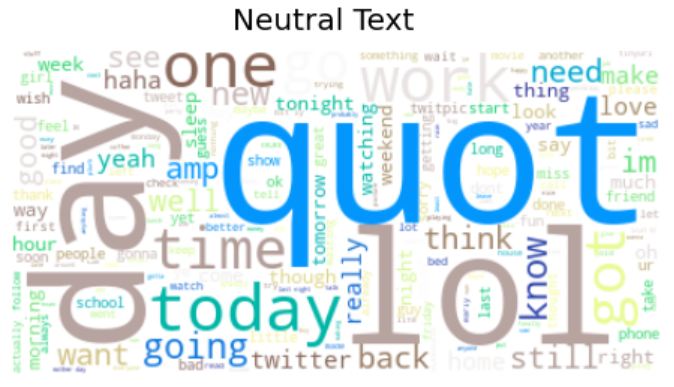
\includegraphics[width=8cm]{neutral_text_wc.png}
\caption{Neutral Text WordCloud}
\end{figure}


Thanks to these word clouds we can see some beautiful information, such as "love" and "mother" being used in the positive texts, while for the negative ones there are a lot of appearences of "sad", "miss" and "work".

To see the real impact those have in the overall results, we should see the most common words in the target. You can see these results in figures \ref{fig:10pos}, \ref{fig:10neg} and \ref{fig:10neu}.

\begin{figure}[!htb]
\centering
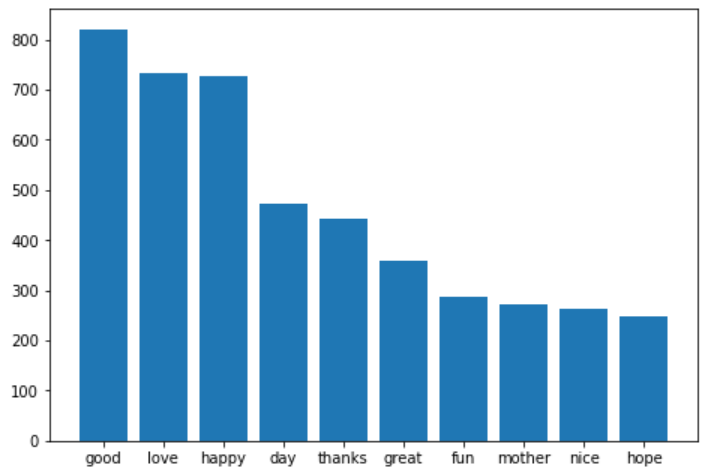
\includegraphics[width=10cm]{top_pos_words.png}
\caption{Top 10 positive selected words}
\label{fig:10pos}
\end{figure}

\begin{figure}[!htb]
\centering
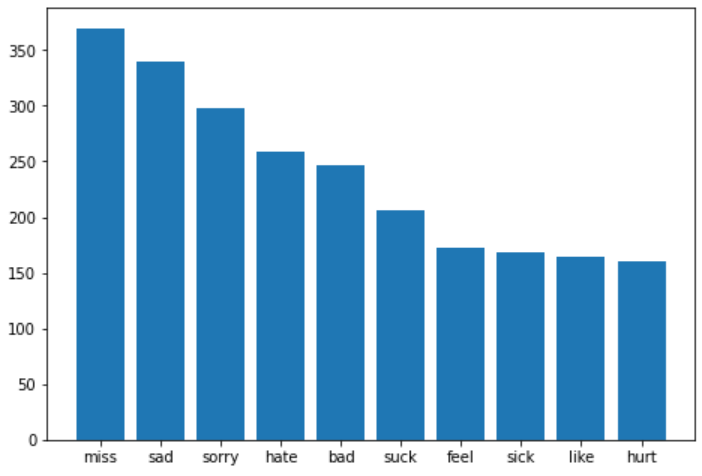
\includegraphics[width=10cm]{top_neg_words.png}
\caption{Top 10 negative selected words}
\label{fig:10neg}
\end{figure}

\begin{figure}[!htb]
\centering
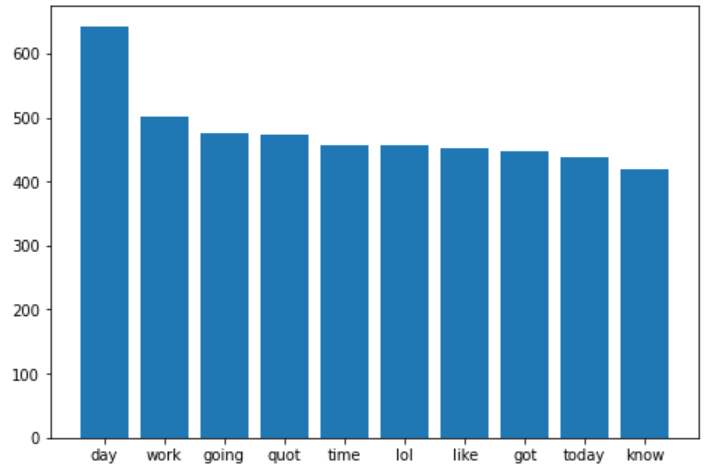
\includegraphics[width=10cm]{top_neu_words.png}
\caption{Top 10 neutral selected words}
\label{fig:10neu}
\end{figure}

What first catches the eye is not that the words that appear are actually the ones most hihglighted in the word clouds, but rather that for the neutral top words (\ref{fig:10neu}), the counts are almost the same for all of them. On the other hand, we see greater variance in the positive and negative charts.

% --------------------
\subsection{Selected Text Length}
% --------------------

Finally, we are going to compare the difference of the lengths between the \textit{text} feature and \textit{selected text} label.

\begin{table}[h]
\centering
\begin{tabular}{c|c|c|c}
\hline
\hline
 & Neutral & Positive & Negative \\ \hline
Text Length Mean & 7.05 & 7.79 & 7.48 \\ 
Selected Text Length Mean & 6.78 & 2.29 & 2.32 \\ 
\hline
\hline
\end{tabular}
\caption{Comparison of text and selected text mean lengths}
\label{tab:text-lengths}
\end{table}

What the results in table \ref{tab:text-lengths} give us are quite interesting. First fo all we see a completely different behavior in positive and negative sentiments vs. neutral, where the mean lengths of both \textit{text} and \textit{selected text} are really close. This means that it is really hard to just select a small subsample of words that carry most of the information about the author's sentiment. However, for positive and negative sentiments it is possible to find key words, which most possibly will be the ones represented with most appearences in the word cloud, as we have already seen by checking the figures \ref{fig:10pos}, \ref{fig:10neg} and \ref{fig:10neu}.

Therefore, as the purpose of this study is to being able to extract these key words, from now on we will disregards the \textbf{neutral} sentiment and focus on obtaining valuable insights for both positive and negative data.

% --------------------
\section{Solution Statement}
% --------------------

We will explore different NLP techniques based on extracting information, explain and apply them.

For the data preprocessing, we will apply the usual tools such as 

\begin{itemize}
    \item \textbf{Lemmatization} - In order to treat as one the different derived forms from a single term. E.g., "friend", "friends" and "friendly" will all be treated as "friend". We are choosing lemmatization over stemming in order to end up with words that NLP techniques can extract meaning from. Note that if we were to use stemming techniques, words would be truncated to their \textit{root} or \textit{stem}, which is the part of the word that contains the global meaning, disregarding derived forms as gender and number. However, it is possible that we end up with words from which algorithms cannot interpret. Taking the word "studies" as an example, its lemma is "study", while the stem is just "studi".
    \item \textbf{Stopwords removal} - Which are terms that lack of their own meaning and are rather user to build up a sentence in a way that it's easier to share its message.
    \item \textbf{Normalize} - Convert all words to lower case.
    \item \textbf{Cleaning} - We've detected selected texts that include some extra added single characters. During the cleaning phase, we will remove words with length 1. We are not afraid of losing any information based on that, as usual one letter words are "a" or "I", so in most cases everything will already be cleaned when removing stop words. Moreover, text just composed by symbols will be removed.
\end{itemize}

After cleaning the data, results will be cached in order to speed up future iterations. Then, we will split the train CSV data into our real train data and validation data as 80 / 20. This gives us 12.933 rows for training and 3.234 for validation after removing the neutral sentiment.

After fitting and comparing results over the validation set applying the Jaccard index, we will compare the performance for the different models.

% --------------------
\section{Benchmark Model}
% --------------------

Our starting point will be \textbf{Named Entity Recognition} as the simplest approach into extracting information from free text.
With the same processed data, we will apply different models and compare their results against NER to see if we can obtain better results.

As the words being used in positive and negative sentiments are really different, we will train a model for each of both sentiments. We will run 10 iterations of the \textbf{spaCy} Python's module to train the data for both positive and negative sentiments.

The obtained results are the following:

\begin{table}[h]
\centering
\begin{tabular}{c|c|c|c}
\hline
\hline
 & Overall & Positive & Negative \\ \hline
Score & 53'62\% & 56'34\% & 50'74\% \\ 
\hline
\hline
\end{tabular}
\caption{NER benchmark results}
\label{tab:bench-results}
\end{table}

And while some of the predictions had full score, sometimes we are just missing by adding or removing words, such as

\begin{verbatim}
    selected_text: I'm thankful
    vs.
    selected_text_pred: thankful
\end{verbatim}

Which gives a 50\% score for that observation.

While we are not obtaining astonishing results, it's not that bad for a benchmark. Also, these numbers went up almost 9 points after our preprocess, as training the model with the raw dataset gives a rough 44\% score. Therefore, we are confident when moving on that our preprocessing is going to be a useful tool.

Finally, what it is really interesting about the NER approach, rather than its implementation, is the underlying logic behind the scenes. It can all be distilled down to letting the algorithm understand the grammatical meaning of a term in a sentence. Therefore, NER is able to identify nouns, verbs, adjectives, etc. These results are based on trying to understand two abstract layers on top of the free text that are nothing but human constructs:
\begin{itemize}
    \item The inherent meaning of a series of characters: a word.
    \item The part this word plays when used together with others to create a sentence.
\end{itemize}


% --------------------
\section{Aspiring Model}
% --------------------

For the aspiring model, we won't be using an out of the box solution such as \textbf{spaCy}'s NER. Moreover, we will be using a totally different logic, which is one of the most interesting aspects of NLP, there are multiple approaches able to solve the same problem.

Again, we won't be focusing in the algorithm implementation, but rather have a brief discussion on the new logic that we are going to apply. Instead of treating this problem with pure linguistics - based on meaning and grammar of words - we will be using trying to answer a question: Given a \textbf{question}, the \textit{sentiment} of each tweet, and a \textbf{context}, the full tweet \textit{text} we want to obtain an \textbf{answer}: the \textit{selected text} label.

% --------------------
\subsection{Question Answering}
% --------------------

This approach tries to formalize how we extract information from text data based on finding the answer of a question which leads us to the problem target. The answer of the question is then present into the \textbf{context}, the text sample.

The model that we are going to use is \textbf{DistilBERT}, a Neural Network that has already been fine-tuned on top of the \href{https://rajpurkar.github.io/SQuAD-explorer/}{Stanford Question Answering Dataset}. Only because of the usage of transfer learning, we can already expect to obtain better results than with NER.

In order to make the training work here, we needed to apply a small extra preprocessing step. The model was failing when it was not able to find the answer by looking into the context. Checking at the raw data, this happened when the \textit{selected text} feature was not correctly informed. We removed 143 rows based on this.

The model has been trained for 3 epochs with a learning rate of 5e-5. We have obtained the following results:

\begin{table}[h]
\centering
\begin{tabular}{c|c|c|c}
\hline
\hline
 & Overall & Positive & Negative \\ \hline
Score & 59'29\% & 60'4\% & 58'12\% \\ 
\hline
\hline
\end{tabular}
\caption{Question-Answer results}
\label{tab:bench-results}
\end{table}

Comparing these number against the benchmark mode, our assumption that using a pretrained model would allow for better scoring held. Also, we are again obtaining slightly better results for positive sentiments than for negative.

Moreover, with Question-Answer we did not need to train separate models for each sentiment, but this might be because of the usage of a pretrained model.

% --------------------
\section{Conclusion}
% --------------------

We have explored two completely different techniques to solve the same problem: extract the subset of a text that contains the sentiment information about the author. In order to achieve this, we have preprocessed the text to normalize the data as much as possible without losing any valuable information.
Moreover, thanks to the data exploration, we discussed how neutral sentiment did not give us any reason to apply any sophisticated method for inferring the target, as most of the text was already being considered as carrier of the sentiment information.
Therefore, both models: NER and Question-Answer have been trained on top of the same cleaned data and validated on a separate partition, which allows us to compare performances.

For the Question-Answer model, we have taken advantage of transfer learning to make it easier to obtain higher quality results. In the end, the aspirant model beat the benchmark placed by NER.

The biggest challenge of the study has been exploring all the different NLP techniques that could be applied on top of our problem. Tackling them from an amateur background on NLP has not been easy, but the wide variety of possible options is what makes NLP most interesting. It is impressive how we can state really simple theoretical ideas that then get translated into algorithms.

The most straight forward improvement in the study would be to deepen the knowledge on how the actual algorithms are built. After that, we would be in a well-suited position to fine tune the results. However, this aspect has been disregarded now as our prime objective was exploring different approaches.

% --------------------
\section{References}
% --------------------

\begin{itemize}
    \item Examples of model implementations have been extracted from the Kaggle's notebooks of the competition. We would like to highlight the following: \href{https://www.kaggle.com/rohitsingh9990/ner-inference-using-spacy-lb-0-628}{NER inference using Spacy}.
    \item \href{https://blog.bitext.com/what-is-the-difference-between-stemming-and-lemmatization/}{What is the difference between stemming and lemmatization}.
    \item \href{https://medium.com/@cristhianboujon/how-to-list-the-most-common-words-from-text-corpus-using-scikit-learn-dad4d0cab41d}{Get the most common words in a corpus}.
    \item \href{https://www.kaggle.com/jonathanbesomi/question-answering-starter-pack}{Question-Answering Starter Pack}.
\end{itemize}

\end{document}
